\section{De JSON-LD a RDF}

La conversión de JSON-LD a RDF es un proceso directo. El sujeto (en JSON-LD), que podría ser usado como objeto en otra tripla, es definido por la propiedad @id, todas las demás propiedades son convertidas en predicado del objeto RDF resultante. Finalmente, los valores literales son extraídos directamente de la propiedad o del valor @value de la propiedad (si lo tuviere). Una propiedad puede tener también definido el lenguaje (@language) y/o tipo de informacion (@type).

Por ejemplo en la figura \ref{img:EjemploBaranJSONLD} se muestra un objeto JSON-LD, que posee un contexto definido dentro del mismo objeto, este contexto también podría estar definido dentro de un documento diferente y referenciado a través de una URI. Tomemos como ejemplo la propiedad foaf:name, la misma se convierte en predicado y el objeto toma el valor del literal “Benjamin Baran” definido en el idioma inglés según especifica @language.



\begin{figure}[h!]
    \centering
    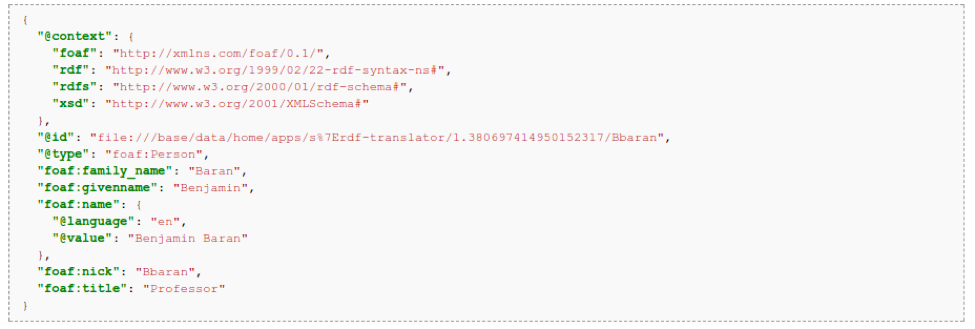
\includegraphics[width=150mm]{figuras/BaranJSONLD.png}
    \caption{Objeto JSON-LD}
    \label{img:EjemploBaranJSONLD}
    \end{figure}




\begin{figure}[h!]
    \centering
    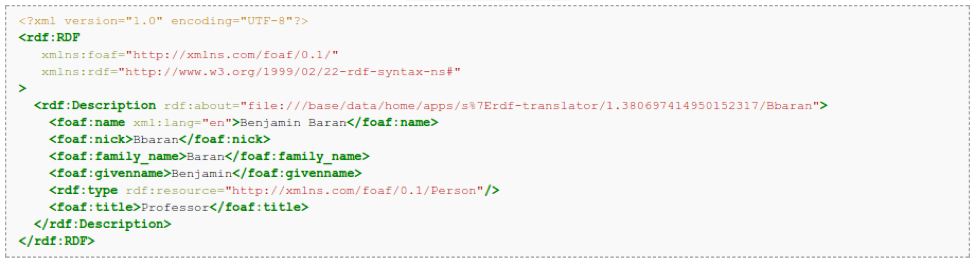
\includegraphics[width=150mm]{figuras/BaranRDF.png}
    \caption{Grafo RDF}
    \label{img:EjemploBaranRDF}
    \end{figure}



